In this section are discussed the details about the implementation of the system, showing a possible (but not unique) implementation plan, an unit and integration testing strategy and some useful DevOps practices that could ease and speedup all the system development process


\subsection{Implementation Plan}
As shown in the Figure~\ref{fig:UML_comp_general} there are three macro component to implement from scratch. The other components either are up and running (i.e.~a Map Service) or were already developed and the only step to do is setup, configure, deploy them. These components will be tested along the developed components in the Integration testing part.

The three macro-components to implement are the CLup User Application, the CLup Server and the Store System. Because all the common interfaces were previously specified (See section~\ref{sect:requirement_traceability}) each of these three components could be implemented independently. This allows three different teams to work in parallel in the implementation of each macro component speeding up the development process.
Even though a full parallel implementation reduces the overall development time in this section will be presented a plan that aims to develop and test the core features of the system and then expands these features. This strategy reduces the time to prototype and time to market of the system and enables the opportunity of doing an alpha test of the system running in a real context, even if the features initially offered are reduced. A secondary objective of the presented plan is to schedule in a smart way the development of the components in order to reduce the number \textit{drivers} and \textit{stubs}. This decision reduces the testing code size while not hindering the quality of the tests.

Therefore the proposed implementation is divided in different iterations. The first iteration aims to produce a working system, the output of the first iteration is, in fact, a full stack working prototype of the system with only the core features. The second iteration refines the features presented in the first iteration and add other important future, in this iteration new component will be integrated to the system and optionally some components already developed in the first iteration are expanded. The successive iterations add quality of life features and polish the system that at the end will be ready for the system test before the release.

For each iteration a graph will show the precedence relations between the components developed or refined during that iteration

\textbf{First Iteration}

\medskip

\begin{figure}[H]
    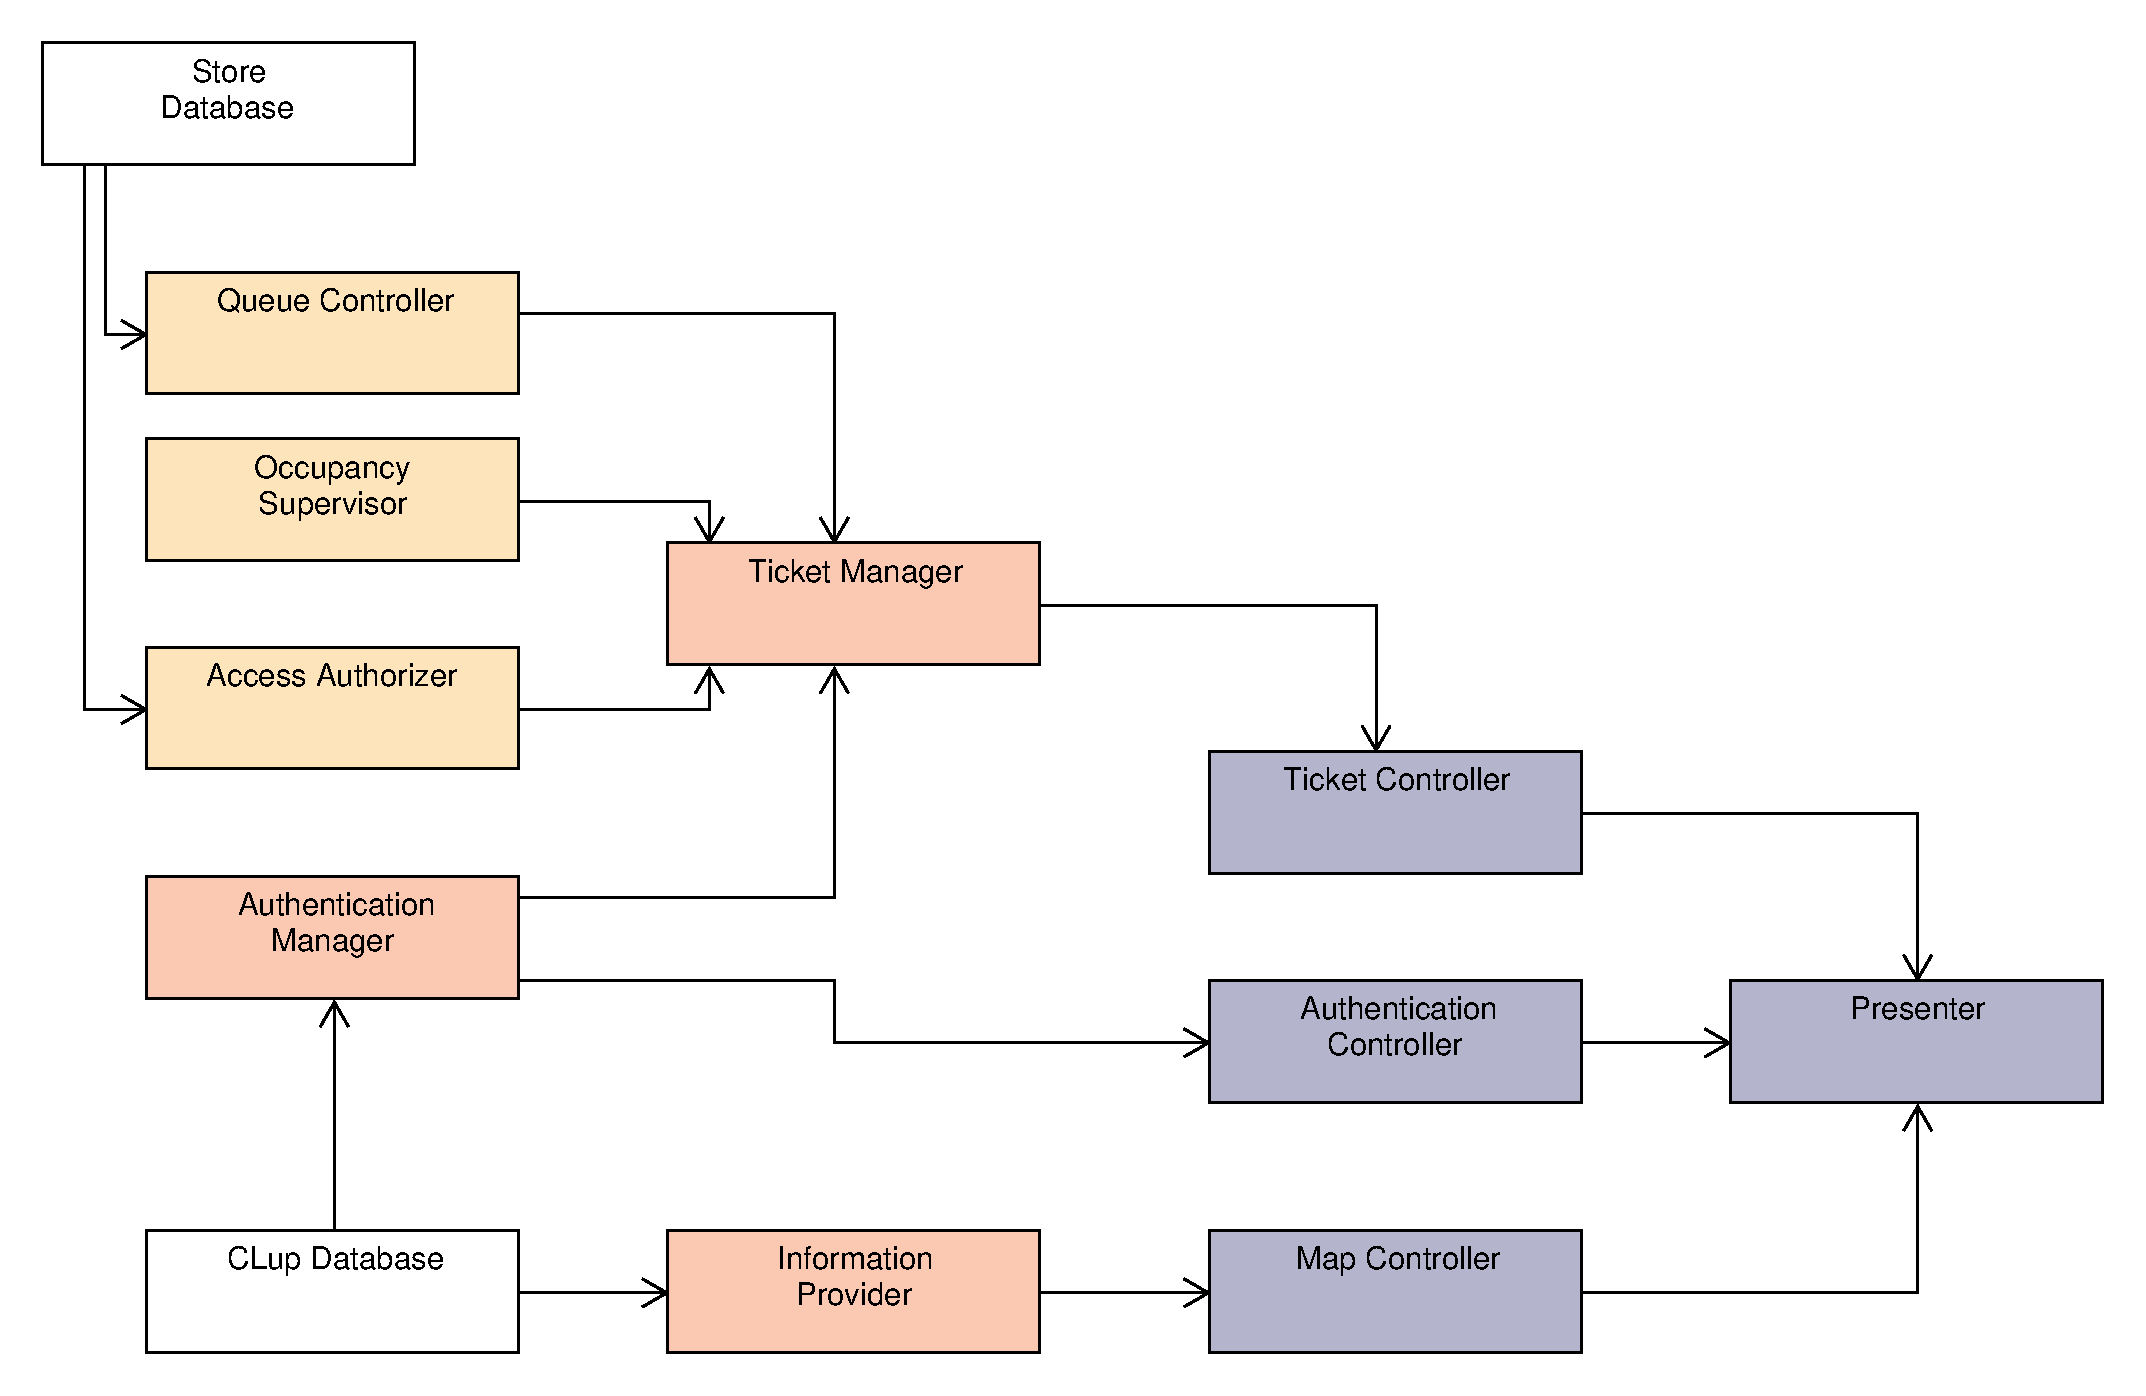
\includegraphics[width=\textwidth]{Images/Impl_Plan_1.pdf}
    \caption{\label{fig:UML_virtual_ticket_sequence}First Iteration of Implementation Plan}
\end{figure}

\textbf{Second Iteration}

\medskip

\begin{figure}[H]
    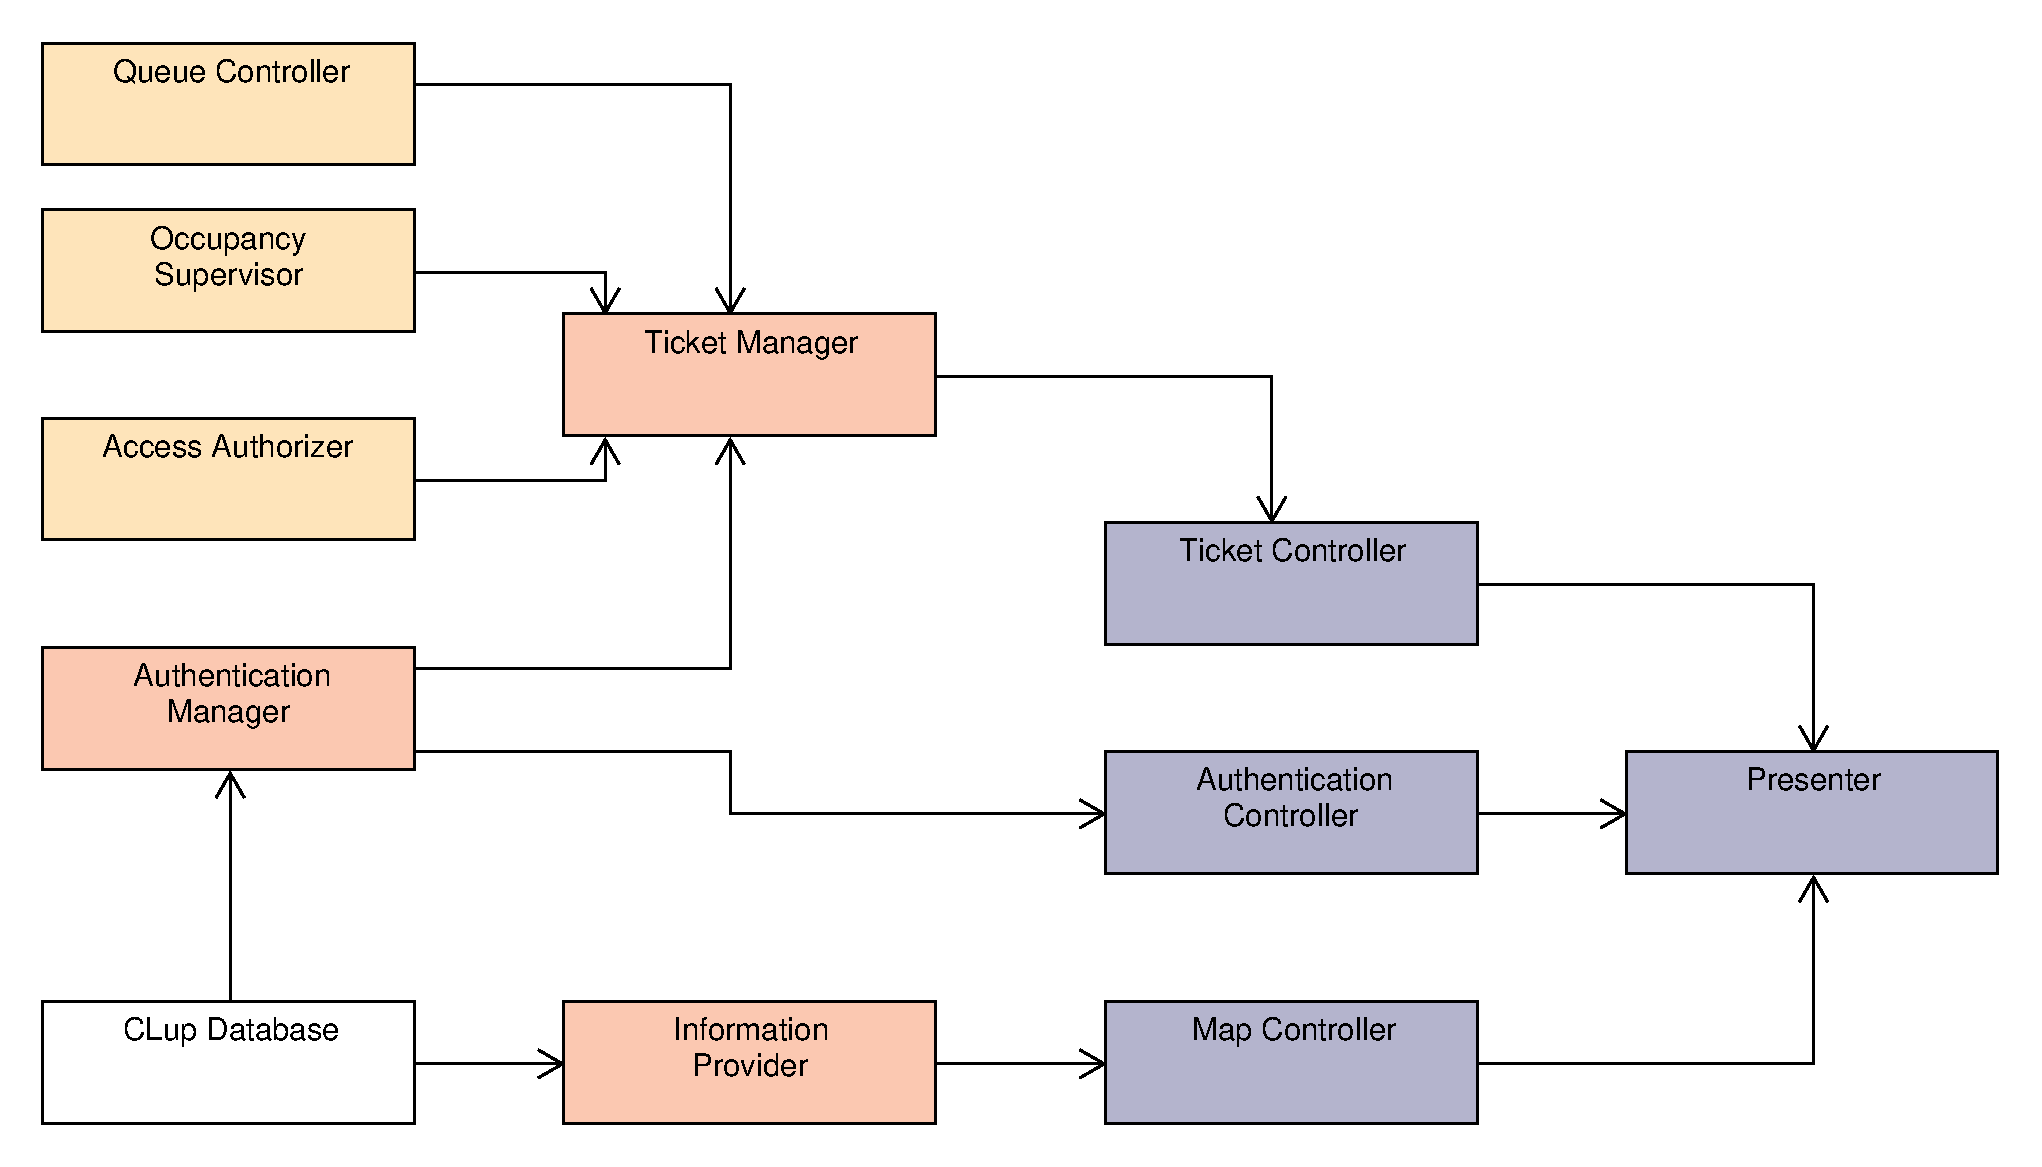
\includegraphics[width=\textwidth]{Images/Impl_Plan_2.pdf}
    \caption{\label{fig:UML_virtual_ticket_sequence}Second Iteration of Implementation Plan}
\end{figure}


\subsection{Unit Testing}
Each component will be developed using mainly the Test Driven Development (TDD) strategy. This strategy consist in writing the unit test cases code before writing the application code forcing the developer to use black box testing over white box testing. In this way the developer has to think at all combinations of the inputs before writing the code. When or after writing the code the developer can always add some white box test case if they feel that this addition could improve the coverage and the effectiveness of the test cases.

The unit testing could be easily performed independently of the programming languages chosen to implement the system because nowadays almost all the mainstream languages provide a unit testing library.
